%\let\uppercase\relax

\vspace{24pt}

\chapter[\textbf{Conclusion}]{Conclusion}

The initial goal of this research project was to continue the work of Dr.\ Matt Terry's thesis by reconstructing his automatic tuner and then investigating target design.  Over time, however, this project has transformed into a more automation focused one, spurred on by the many common computational tasks involved in shock timing.  

This departure from creating a single-purpose automatic tuner used for investigating target design has led to many tools with relevance outside of shock ignition and even of inertial fusion. AHAB, for example, was constructed because the original automatic tuner was unsalvageable.  Although its use for this project was limited to timing the picket pulse and the pedestal pulses (see Fig.\,\ref{fig:shockConverge}), it could be used to automate the entire shock timing process.  This would increase the scope of research problems to ones requiring multiple tuned laser profiles, such as the design of fuel targets.

\sidecaptionvpos{figure}{c}
\begin{SCfigure}[][h!]	
	\centering
	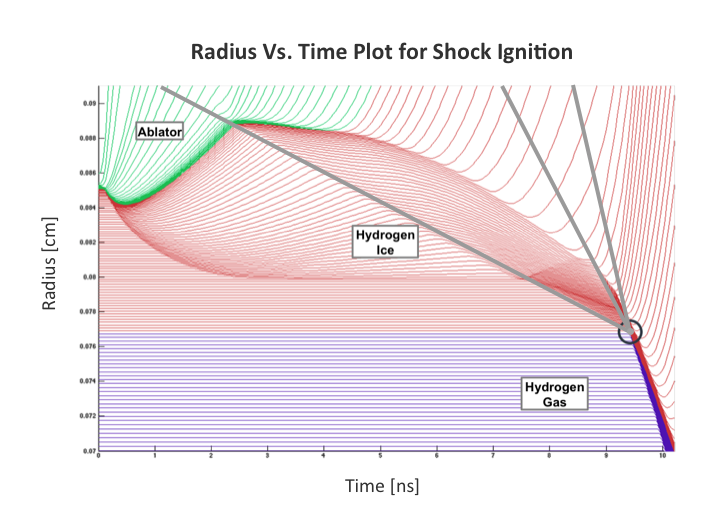
\includegraphics[width=.72\textwidth]{graphics/shockConverge.png} 
	\caption[Shock Convergence]{ The \\ Convergence of the Three Pedestal Pulses \\ \captiontitlefinal{\textmd{at the ice-gas boundary of the Hydrogen fuel source. This type of plot is discussed in Appendix\,\ref{app:rtt}.  The main point to take from it is that on a Radius Vs. Time plot, the three drawn lines represent the resulting shocks' wave speeds. } } }
	\label{fig:shockConverge}
\end{SCfigure}

In order to develop an automatic tuner, though, another program would be needed.  This program, currently codenamed Mobile Operating Batch Inspector (MOBI), would be sent to HTCondor and would then submit multiple instances of AHAB.  Further, because laser profile construction is iterative, each new laser segment could be written to its own input section, see 'Loading Multiple Input Decks from One File' in Appendix\,\ref{app:restart}.   

The first step in developing this automatic tuner would be to quantify the accuracy of shock timing.  This could be done by introducing a new parameter -- the shock breakout -- that could be inspected by MOBI in post-processing to guide future AHAB submissions.  This would prevent the need for human interpretation and interaction, both of which were used to construct the profile in Fig.\,\ref{fig:shockConverge}.

For timing the shocks, the term \textit{shock breakout} refers to when the outermost Hydrogen gas layer reaches a velocity of 3.5e5 cm/s \citep{terryThesis}.  Using this method, each new shock would have its shock breakout time plotted against its launch time.  Because a late-arriving shock would not alter this breakout time, the optimal time to start would, then, be when the breakout time just starts to move, see Fig.\,\ref{fig:shockBreakout}.

\sidecaptionvpos{figure}{c}
\begin{SCfigure}[][h!]	
	\centering
	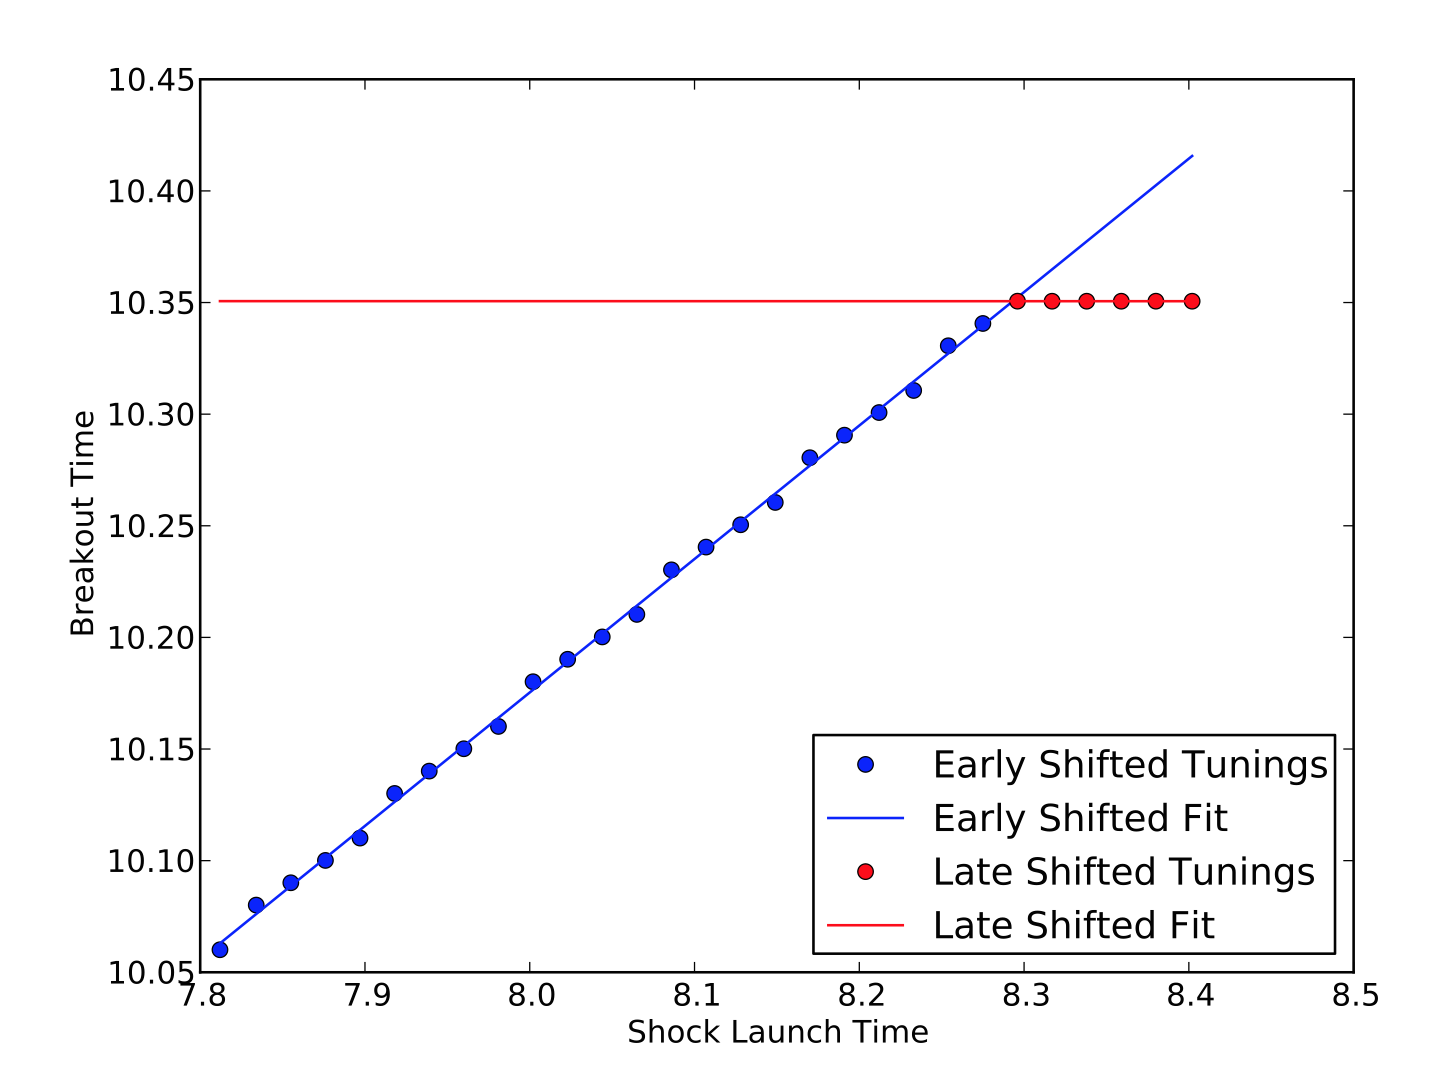
\includegraphics[width=.621\textwidth]{graphics/shockBreakout.png} 
	\caption[Automatically Timing Pedestal Pulses]{ \\ Timing a Pedestal Pulse \\ \captiontitlefinal{\textmd{requires finding the intersection between the positively sloped region of the breakout time curve and the horizontal region of it.  This is done by varying the shock launch time and measuring the resulting breakout time \citep{terryThesis}. } } }
	\label{fig:shockBreakout}
\end{SCfigure}
\sidecaptionvpos{figure}{b}

As mentioned in Sec.\,\ref{sec:mainPulses}, the compression pulse and the igniter pulse require optimizing some variable.  Although these optimized variables were stated as the target density and the energy yield, respectively, each optimized quantity could be further complicated by investigating multiple properties simultaneously.  This could include: increasing a pulse effect's robustness, achieving certain value requirements, and developing new parameters to quantize certain physical behaviors \citep{terryThesis,perkinsPaper,picketPaper}.  

Although some other unforeseen tools and analytics will be needed, AHAB should now be in a state that allows integration into a program like MOBI without too much modification.  To make sense of the Bucky output along the way, the Radius, Time, and Temperature Plot discussed in Appendix\,\ref{app:rtt} will prove to be invaluable.